\section{Greenhouse Model}
\begin{figure}[H]
	\centering
	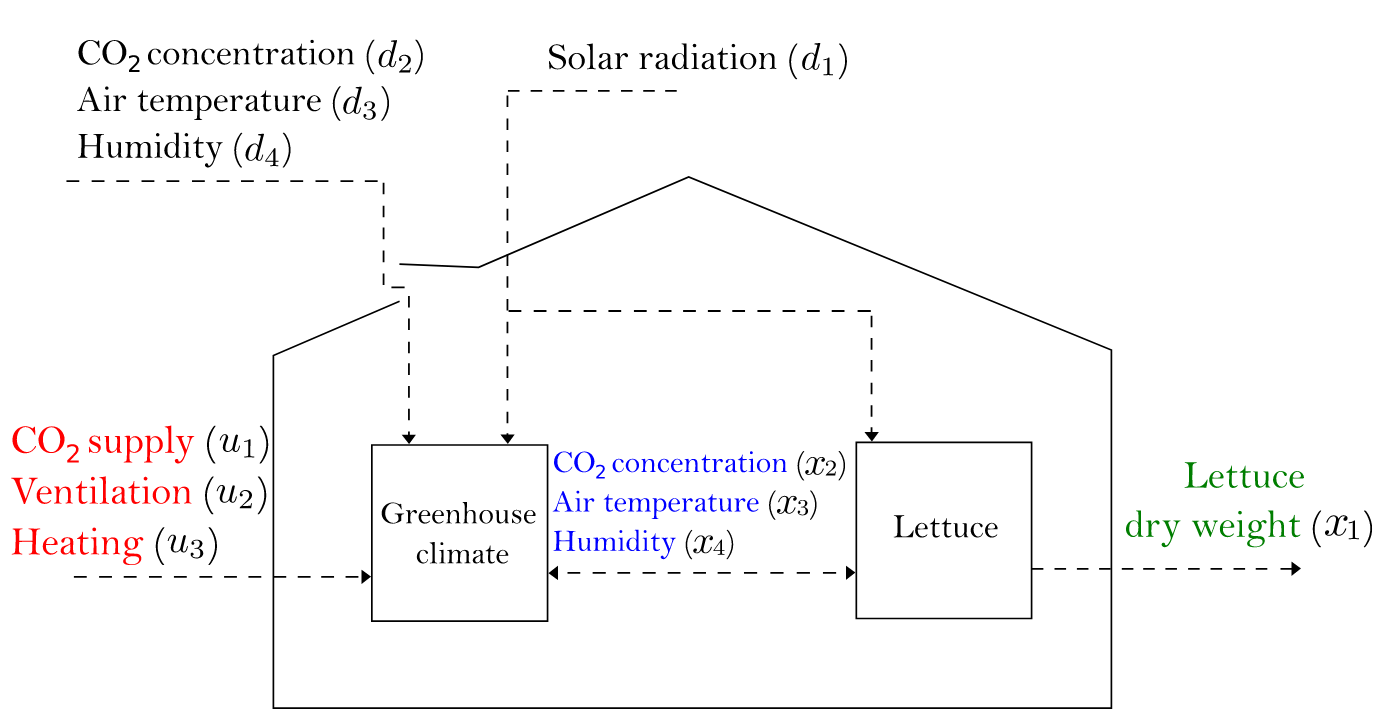
\includegraphics[width = \linewidth]{figures/van_henten_model.png}
	\caption{Graphical representation of greenhouse crop production \cite{hentenGreenhouseClimateManagement1994}}
	\label{fig:van_henten_model}
\end{figure}


\autoref{fig:van_henten_model} displays a graphical representation of the greenhouse model from the works of \citet{hentenGreenhouseClimateManagement1994} and has been used in previous works\cite{morcegoReinforcementLearningModel2023,lubbersAutonomousGreenhouseClimate2023, boersmaRobustSamplebasedModel2022}. The control inputs are highlighted in red, the states of the indoor climate in blue, the state of the crop in green and the external weather disturbances in black. The model was discretised with the fourth order Runge-Kutta Method with a sample period $\Delta t = 30$ min, resulting in the following system dynamics:
\begin{equation}\label{eq:greenhouse_model_discrete}
	\begin{aligned}
		& x(k+1) = f(x(k),u(k),d(k),p) \\
		& y(k) = g(x(k),p)
	\end{aligned}
\end{equation}
with discrete time $k \in Z^{0+}$, state variable $x(k) \in \mathbb{R}^4$, measurement $y(k) \in \mathbb{R}^4$, control input $u(k) \in \mathbb{R}^3$ and weather disturbance $d(k) \in \mathbb{R}^4$. The parameter $p \in \mathbb{R}^{28}$ represents all parameters used in the model, with $f(\cdot)$ and $g(\cdot)$ as the system's non-linear functions. The states of the system, control inputs, disturbances and outputs are described below.

\begin{equation}
	\begin{aligned}
		& x(k) = \begin{bmatrix}
			x_1 & x_{2} & x_3 & x_4
		\end{bmatrix}^T
		\\
		& u(k) = \begin{bmatrix}
			u_{1} & u_{2} & u_3
		\end{bmatrix}^T
		\\
		& d(k) = \begin{bmatrix}
			d_{1} & d_{2} & d_3& d_4
		\end{bmatrix}^T
		\\
		& y(k) = \begin{bmatrix}
			y_1 & y_{2} & y_3 & y_{4}
		\end{bmatrix}^T
	\end{aligned}
	\label{eq: model vectors}
\end{equation}

The measured output is essentially the same as the state of the system; however, the units of the indoor $C0_2$ density ($y_2$) and relative humidity ($y_4$) differ in that they report in units used in standard measurement sensors.

\begin{figure}[H]
	\centering
	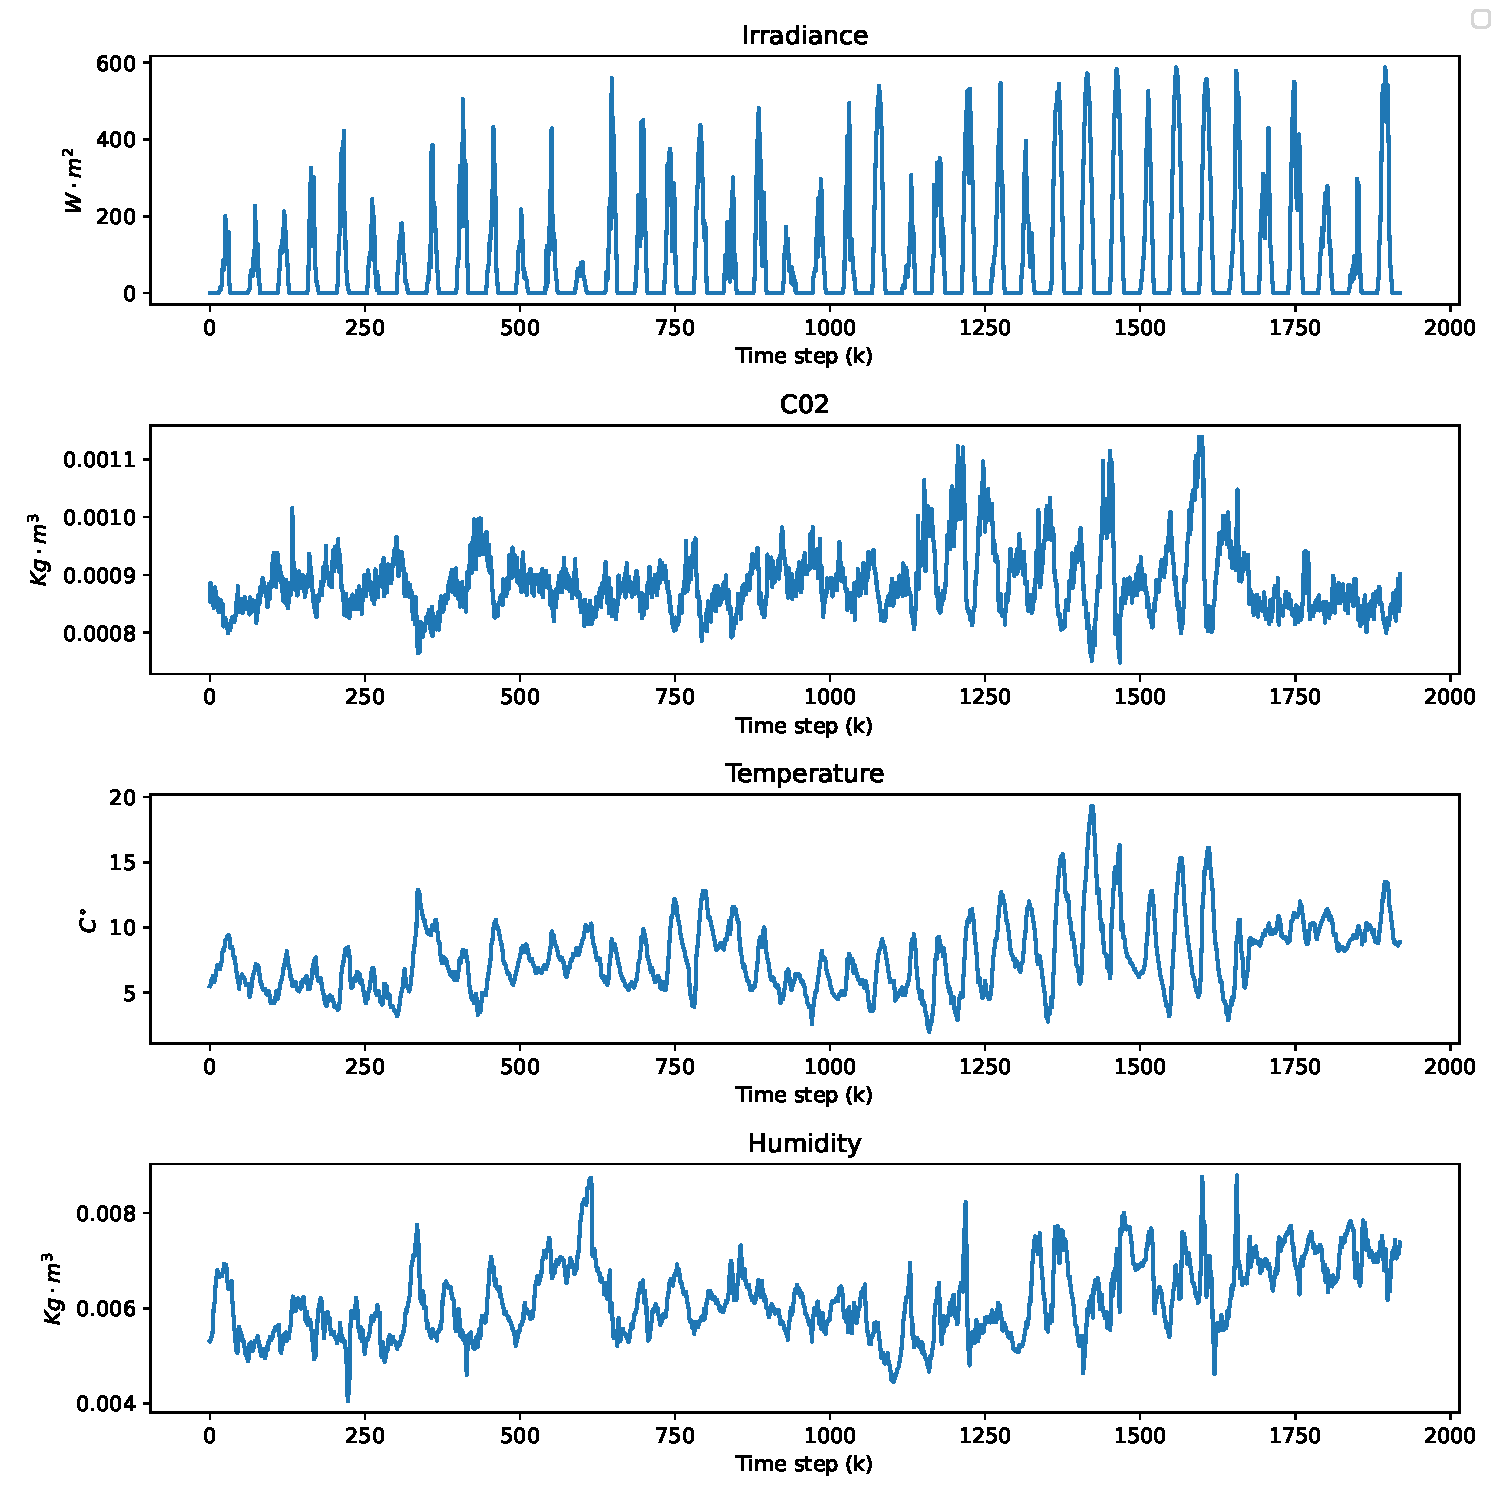
\includegraphics[width=\linewidth]{figures/weather_data_vertical.pdf}
	\caption{Weather Data}
	\label{fig:weather-data}
\end{figure}

The weather data for simulations and training was sourced from the Venlow Greenhouse in Bleiswijk, covering the period from January 30 to March 11, 2014. The weather is assumed to be deterministic and known at each time step. This dataset, shown in \autoref{fig:weather-data}, spans a 40-day growing period with a time step of 30 minutes, resulting in a total of 1920 time steps.



\subsection{Model Uncertainty}
As done in \cite{boersmaRobustSamplebasedModel2022, lubbersAutonomousGreenhouseClimate2023}, the source of uncertainty in the stochastic environment is modeled as parametric uncertainty, aiming to capture all the uncertainties in the greenhouse environment. The parameters of the environment are represented as uncertain with well-defined probabilistic properties. It is assumed that the uncertain parameters, $\hat{p}$, follow a uniform probabilistic distribution:

\begin{equation}
	\label{eq:uncertainty_model}
	\begin{aligned}
		\hat{p} \sim U(\mu_p, \delta)  
	\end{aligned}
\end{equation}

where $\mu_p$ is the mean value of the parameters and $\delta_p$ is expressed as a percentage such that the upper and lower bounds of the distribution is expressed as $p(1-\delta_p)$ and $p(1+\delta_p)$. This was done to guarantee that the sampled model parameters are always non-negative. Since all parameters are perturbed, including parameters of the output measurement equations, output noise is also introduced. Introducing this uncertainty results in the following system dynamics:

\begin{equation}\label{eq:greenhouse_model_discrete_uncertain}
	\begin{aligned}
		& \hat x(k+1) = f(\hat x(k),u(k),d(k),\hat p(k)) \\
		& \hat y(k) = g(\hat x(k),\hat p(k))
	\end{aligned}
\end{equation}

where the states and output measurements of the system are uncertain and $\hat{p}(k)$ denotes the uncertain parameters and is resampled at every time step.

\subsection{Optimization Goal}
To directly optimize the economic profit of the greenhouse, it is essential to maximize lettuce size while minimizing resource usage during its growth period, considering the pricing of energy and lettuce. This is referred to as the Economic Profit Indicator (EPI), and optimizing it forms the basis of the following optimization objective:

\begin{equation}\label{eq:epi}
	\min_{u_1,u_3}\sum_{k = t_s}^{t_f} (c_{p_1} \cdot u_1(k) + c_{p_2} \cdot u_3(k))\cdot \Delta t - c_{p_3} \cdot y_1(t_f)
\end{equation}

where $t_s$ denotes the start time of the growth period, $t_f$ the end time, $\Delta t$ the sample time interval,$c_{p1},c_{p2}$ the pricing coefficients of injecting $C0_2$, and heating, respectively and $c_{p3}$ as the price of lettuce. These pricing factors are shown in \autoref{tab:pricing_factors}. It is important to highlight that ventilation, such as opening windows, does not incur any costs and, therefore, does not have a pricing factor. $t_s$ and $t_f$ was selected so that the growing period is fixed at 40 days.\\
However, this optimization goal makes the reward incredibly sparse, making it difficult to optimize directly with both MPC and RL. Consequently, a stage cost received at every time interval is used, where the total sum of these stage costs throughout the growing period corresponds to the optimization objective in \autoref{eq:epi}. Therefore, the optimization goal that RL, MPC, and RL-MPC aim to optimize is:

\begin{subequations} \label{eq:optimisation-goal}
	\begin{align}
		& \min_{u_1,u_3} \sum_{k = t_s}^{t_f} \left[ l(y(k),u(k)) \right] \label{eq:stage-cost-epi} \\
		\text{s.t.} \quad 
		& \hat{x}(k+1) = f(\hat{x}(k), u(k), d(k), \hat{p}(k)), \label{eq:constraint-1} \\
		& \hat{y}(k) = g(\hat{x}(k+1), \hat{p}), \label{eq:constraint-dynamics} \\
		& -\delta u_{max} \leq u(k) - u(k-1) \leq \delta u_{max}, \label{eq:constraint-delta-u} \\
		& u_{\min} \leq u(k) \leq u_{\max}, \label{eq:constraint-u-limits} \\
		& x(k_0) = x_{k_0}. \label{eq:constraint-initial}
	\end{align}
\end{subequations}

where 
\begin{equation}
	l(y(k),u(k)) = (c_{p_1} \cdot u_1(k) + c_{p_2} \cdot u_3(k)) \cdot \Delta t  - c_{p_3} \cdot (y_1(k) - y_1(k-1))
\end{equation}
where the constraints are detailed below:
\begin{equation}\label{eq:constraints}
	\begin{aligned}
		&u_{min} = \begin{pmatrix}
			0&0&0
		\end{pmatrix}^T \\
		&u_{max} = \begin{pmatrix}
			1.2&7.5&150
		\end{pmatrix}^T	\\
		& \delta u_{max} = \frac{1}{10} u_{max}\\
		&y_{min} = \begin{pmatrix}
			0&500&10&0
		\end{pmatrix}^T \\
		&y_{max} = \begin{pmatrix}
			\infty&1600&20&100
		\end{pmatrix}^T	\\
	\end{aligned}
\end{equation}

The values in \autoref{eq:constraints} were obtained from typical horticultural practices and previous works \cite{boersmaRobustSamplebasedModel2022,morcegoReinforcementLearningModel2023,jansenOptimalControlLettuce2023}. 

\begin{table}[H]
	\centering
	\begin{tabular}{|c|c|c|}
		\hline
		\textbf{Symbol} & \textbf{Value} & \textbf{Units} \\
		\hline
		$c_{p_1}$ & $1.906\cdot 10^{-7} \times 10^{-4}$ & $ \text{\euro} \cdot mg^{-1}$ \\
		$c_{p_2}$ & $3.558 \times 10^{-8}$ & $ \text{\euro} \cdot J^{-1}$ \\
		$c_{p_3}$ & $22.285$ & $\text{\euro} \cdot kg^{-1}$ \\ 
		\hline
	\end{tabular}
	\caption{Pricing factors}
	\label{tab:pricing_factors}
\end{table}